\providedisablepart{showscreenshot}
\begin{frame}[fragile]
    \def\mybox#1{\square_{#1}}
    \def\mydia#1{\lozenge_{#1}}
    \def\sfiven{{S5_n}}
    \frametitle{Example: Epistemic Q\&A}
    \centering
    \strplain{\makebox[9.5cm][l]{John knows that Mary or Eve knows that Ping has a dog.}\makebox[1.5em]{\upshape($S_1$)}\\
              \makebox[9.5cm][l]{Mary doesn't know if Ping has a dog.}\makebox[1.5em]{\upshape($S_2$)}\\
              \makebox[9.5cm][l]{Does Eve know if Ping has a dog?}\makebox[1.5em]{\upshape($Q$)}}

    {\color{logicfont}
        \begin{align*}
            S_1 &= \mybox{john}(\mybox{mary} hd(ping)\vee \mybox{eve}hd(ping))\\
            S_2 &= \neg(\mybox{mary}hd(ping) \vee \mybox{mary}\neg hd(ping))\\
            Q &= \mybox{eve}hd(ping) \vee \mybox{eve}\neg hd(ping)
        \end{align*}
    }

    \begin{table}
        \begin{tabular}{l l}
            $S_1, S_2 \vdash_\sfiven Q$\quad      &$\leadsto$\quad yes\\
            $S_1, S_2 \vdash_\sfiven \neg Q$\quad &$\leadsto$\quad no\\
            else &$\leadsto$\quad maybe
        \end{tabular}
    \end{table}
    \ifpart{showscreenshot}{\only<2>{
        \begin{tikzpicture}[overlay,remember picture]
            \fill[gray!80,opacity=0.8] (current page.north west) rectangle (current page.south east);
            \node at (current page.center) { 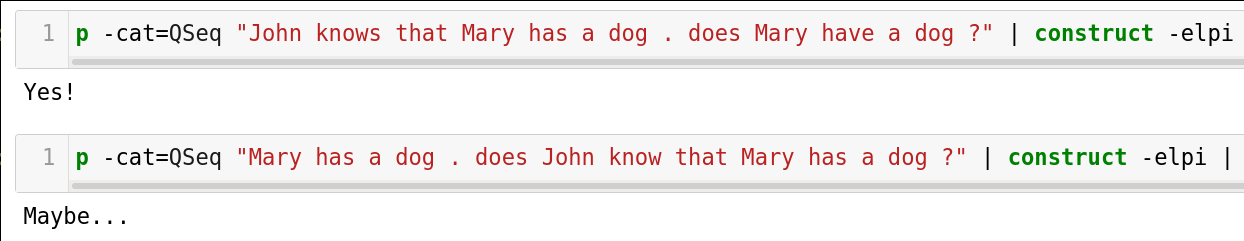
\includegraphics[width=0.9\textwidth]{img/screenshot-glif-4.png} };
        \end{tikzpicture}
    }}{}
\end{frame}
